\begin{tikzpicture}
    % Second column, prior dstirbutions
    \node (d0) {
\includegraphics[width=40pt]{dist_0}};
    \node[below=-10pt of d0] (d1) {
\includegraphics[width=40pt]{dist_1}};
    \node[below=-10pt of d1] (d2) {
\includegraphics[width=40pt]{dist_2}};
    \node[below=-10pt of d2] (d3) {
\includegraphics[width=40pt]{dist_3}};
    \node[above=-9pt of d0] (td) {\(p(\s_i)\)};

    % First columns, data
    \node[left=30pt of d0] (s0) {
\includegraphics[width=25pt]{mixing/bass.png}};
    \node[left=30pt of d1] (s1) {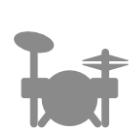
\includegraphics[width=25pt]{mixing/drums.png}};
    \node[left=30pt of d2] (s2) {
\includegraphics[width=25pt]{mixing/voice.png}};
    \node[left=30pt of d3] (s3) {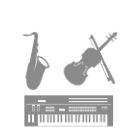
\includegraphics[width=25pt]{mixing/other.png}};
    \node[above=0pt of s0] (ts) {data};

    % Arrows frist to second
    \draw [->] (s0) to (d0);
    \draw [->] (s1) to (d1);
    \draw [->] (s2) to (d2);
    \draw [->] (s3) to (d3);
    \draw (ts) -- (td) node [above, midway,align=center] {estimate};

    % Column posterior
    \node[right=30pt of d0] (dp0) {
\includegraphics[width=40pt]{dist_0_post}};
    \node[right=30pt of d1] (dp1) {
\includegraphics[width=40pt]{dist_1_post}};
    \node[right=30pt of d2] (dp2) {
\includegraphics[width=40pt]{dist_2_post}};
    \node[right=30pt of d3] (dp3) {
\includegraphics[width=40pt]{dist_3_post}};
    \node[above=0pt of dp0] (tp) {posterior};

    % Mix wave
    \node[above right=10pt of td] (wav) {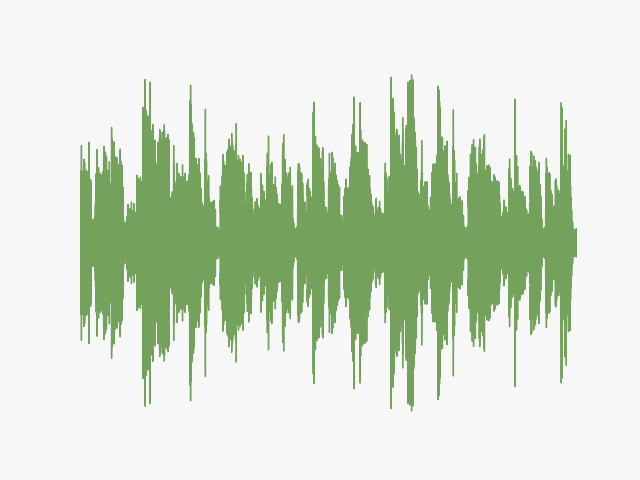
\includegraphics[width=40pt]{mixing/mix_wav.png}};
\end{tikzpicture}
